\documentclass[xcolor=pdftex,table,10pt]{beamer}

\mode<presentation> {
  \usetheme{Madrid}
  \usecolortheme{seahorse}
  \usecolortheme{rose}
}

\AtBeginSection[]
{
  \begin{frame}<beamer>
    \frametitle{Outline}
    \tableofcontents[currentsection,hideothersubsections]
  \end{frame}
}

\AtBeginSubsection[]
{
  \begin{frame}<beamer>
    \frametitle{Outline}
    \tableofcontents[currentsection,currentsubsection]
  \end{frame}
}

%change bottom line
\setbeamertemplate{footline}
{
  \leavevmode%
  \hbox{%
  \begin{beamercolorbox}[wd=.23\paperwidth,ht=2.25ex,dp=1ex,center]{author in head/foot}%
    \usebeamerfont{author in head/foot}\insertshortauthor
  \end{beamercolorbox}%
  \begin{beamercolorbox}[wd=.54\paperwidth,ht=2.25ex,dp=1ex,center]{title in head/foot}%
    \usebeamerfont{title in head/foot}\insertshorttitle
  \end{beamercolorbox}%
  \begin{beamercolorbox}[wd=.23\paperwidth,ht=2.25ex,dp=1ex,right]{date in head/foot}%
    \usebeamerfont{date in head/foot}\insertshortdate{}\hspace*{2em}
    \insertframenumber{} / \inserttotalframenumber\hspace*{2ex} 
  \end{beamercolorbox}}%
  \vskip0pt%
}

\usepackage[english]{babel}
\usepackage[latin1]{inputenc}
\usepackage{times}
\usepackage{listings}
\usepackage{colortbl}
\usepackage{tikz}
\usepackage{verbatim}
\usepackage{algorithm}
\usepackage{algorithmic}
\usepackage{amsmath}
\usepackage{amsfonts}
\usetikzlibrary{shapes,arrows,snakes,backgrounds}
\usefonttheme[onlymath]{serif}
%\usepackage[T1]{fontenc}
%\usepackage{color}
%\usepackage[x11names, rgb]{xcolor}
%\usepackage{dot2texi}
%\usepackage{pgfplots}
%\usefonttheme{professionalfonts}

\newcommand{\opal}{\textsc{OPAL }}
\renewcommand {\Re}{{\mathbb{R}}}

\title{A Parallel Multigrid Solver for Beam Dynamics}
\author{Yves Ineichen (ETH Zurich)}
\institute{\textbf{Master Thesis} \\ Supervisor: Andreas Adelmann (PSI) \\ Supervising Professor: Peter Arbenz (ETH)}
\date{14th August 2008}
%\logo{
\includegraphics[width=3cm]{psilogo}}
\titlegraphic{
	\begin{columns}
		\begin{column}{3cm}
			\includegraphics[width=2cm]{ethlogo} \\
		\end{column}
		\begin{column}{2cm}
			
\includegraphics[width=3cm]{psilogo} \\
		\end{column}
	\end{columns}
}

\begin{document}

% For every picture that defines or uses external nodes, you'll have to
% apply the 'remember picture' style. To avoid some typing, we'll apply
% the style to all pictures.
\tikzstyle{every picture}+=[remember picture]

% By default all math in TikZ nodes are set in inline mode. Change this to
% displaystyle so that we don't get small fractions.
\everymath{\displaystyle}

	\lstset{language=C++, basicstyle=\small}

	\begin{frame}
		\titlepage
	\end{frame}
	
	\begin{frame}
	  \frametitle{Outline}
	  \tableofcontents
	\end{frame}

	\section{Motivation}

	\begin{frame}
		\frametitle{Motivation}
		\framesubtitle{Space-Charge Calculation in \opal I}
		
		\begin{block}{Space-Charge in the Electrostatic Approximation}
			Whenever we have a number of moving charged particles:
			\begin{itemize}
				\item electric fields  caused by Coulomb repulsion are present
				\item magnetic fields arising from the moving particles
			\end{itemize}
		Both effects acts as \alert{forces} on to the particles!	
		\end{block}

		\pause
		\vspace{0.5cm}

		Express the Coulomb potential $\phi$ in terms of charge densities $\rho$ (proportional to the particle density). The electric field can be expressed by 
		\[
			\mathbf{E} = - \nabla \phi \text{.}
		\]
		The arising Poisson's equation for the electrostatic potential has the form
		\[
			\nabla^2 \phi = - \frac{\rho}{\varepsilon_0}\text{.}
		\]

		The Magnetic field can be calculated from the electric field by the Lorentz transformation.
		
		%Solve Maxwell's equation in the non-relativistic bunch frame on the grid
		%\begin{eqnarray*}
		%	\nabla \times \mathbf{E} + \frac{\partial\mathbf{B}}{\partial \mathbf{t}} = \mathbf{0} \\
		%	\nabla \cdot \mathbf{B} = 0
		%\end{eqnarray*}

	\end{frame}
	
	\begin{frame}
		\frametitle{Motivation}
		\framesubtitle{Space-Charge Calculation in \opal II}

		\begin{block}{Particle-in-cell (PIC) Method in N-body Simulations}
		\begin{itemize}
			\item interpolate individual particle charges to the grid
			\item solve the Poisson equation on the mesh in a Lorentz frame
			\item values of the potential at the location of individual particles is interpolated from the potential at the grid points
			\item typically faster $\mathcal{O}(n \log{n})$ than Particle-Particle method $\mathcal{O}(n^2)$
		\end{itemize}
		\end{block}

		\vspace{0.8cm}
		\pause

		We apply a second order finite difference scheme which leads to a set of linear equations
		\[
			\mathbf{A} \mathbf{x} = \mathbf{b} \text{,}
		\]
		where $\textbf{b}$ denotes the charge densities on the mesh.
	\end{frame}

	\begin{frame}
		\frametitle{Motivation}
		\framesubtitle{Space-Charge Calculation in \opal III}

		\begin{exampleblock}{Current space-charge calculation in \opal}
		\begin{itemize}
			\item FFT based direct solver: convolution with Green's function
			\item rectangular domain with open and periodic boundary conditions
		\end{itemize}
		\end{exampleblock}

		\pause
		\vspace{0.2cm}

		\begin{alertblock}{Goals: improvements}
		\begin{itemize}
			\item solve anisotropic electrostatic Poisson PDE with an iterative solver
			\item irregular domain with ``exact'' boundary conditions
		\end{itemize}
		\end{alertblock}

		\pause
		
		\begin{enumerate}
			\item implement a preconditioned iterative solver
			\item incorporate this solver in \opal
			\item handle the irregular boundary points
			\item investigate and implement ways to enable \opal to use exact beam pipe geometries
		\end{enumerate}

	\end{frame}
	
%	\begin{frame}
%		\frametitle{Motivation}
%		\framesubtitle{Problem Formulation}
%
%		\begin{block}{Problem Statement}
%		Solve the anisotropic (Lorentz transformation) electrostatic Poisson PDE on an irregular bounded (motivated by the beam-pipe geometry) domain with an iterative solver.
%		\end{block}
%
%		\pause
%		\vspace{0.9cm}
%
%
%	\end{frame}

    %CONTENT: exp lain mg, sa (short), benefits (AND reusing old solution as approx),
    \section{Solver}

	\begin{frame}
		\frametitle{Multigrid Algorithm}

		%\begin{algorithm}
		%\caption{Multigrid V-cycle Algorithm}
		\begin{block}{Mutligrid V-Cycle Algorithm}
		\begin{algorithmic}[1]
			\STATE \textbf{procedure} MultiGridSolve($A_l$, $b_l$, $x_l$, $l$)

			\IF{$l$ = maxLevel-1}
			    \STATE DirectSolve $A_l \mathbf{x}_l = \mathbf{b}_l$
			\ELSE
			    \STATE $\mathbf{x}_l$ $\leftarrow$ $S^{pre}_l$($A_l$, $\mathbf{b}_l$, $0$)
			    \STATE $\mathbf{r}_l$ $\leftarrow$ $\mathbf{b}_l$ - $A_l \mathbf{x}_l$ \COMMENT{calculate residual}
			    \STATE $\mathbf{b}_{l+1}$ $\leftarrow$ $R_l \mathbf{r}_l$ \COMMENT{Restriction}
			    \STATE $\mathbf{v}_{l+1}$ $\leftarrow$ $\mathbf{0}$
			    \STATE MultiGridSolve($A_{l+1}$, $\mathbf{b}_{l+1}$, $\mathbf{v}_{l+1}$, $l+1$)
			    \STATE $\mathbf{x}_l$ $\leftarrow$ $\mathbf{x}_l$ + $P_l \mathbf{v}_{l+1}$ \COMMENT{coarse grid correction}
			    \STATE $\mathbf{x}_l$ $\leftarrow$ $S^{post}_l$($A_l$, $\mathbf{b}_l$, $\mathbf{x}_l$)
			\ENDIF
			\STATE \textbf{end procedure}
		\end{algorithmic}
		%\end{algorithm}
		\end{block}

	\end{frame}

	\begin{frame}
		\frametitle{Prolongation Operator (1/2)}
		\framesubtitle{Smoothed Aggregation: The Grid Transfer Operator}

		\begin{columns}
		\begin{column}{6.7cm}
			\begin{enumerate}
				\item discretization matrix $A_l$ is converted into a graph $G_l$
				\item assign each vertex of $G_l$ is assigned to one aggregate % of the disjoint aggregate set where each aggregate represents a coarse grid vertex
				\item the tentative prolongation operator matrix is formed 
				\begin{itemize}
					\item matrix rows correspond to vertices
					\item matrix columns to aggregates
					\[
						p_{i,j} = \begin{cases} 1 & \text{if } i^{th} \text{ vertex in } j^{th} \text{ aggregate} \\ 
								        0 & \text{otherwise}
							  \end{cases}
					\]
				\end{itemize}
				\item improve robustness by smoothing the tentative prolongation operator

			\end{enumerate}
		\end{column}

		\begin{column}{4cm}
			\begin{center}
				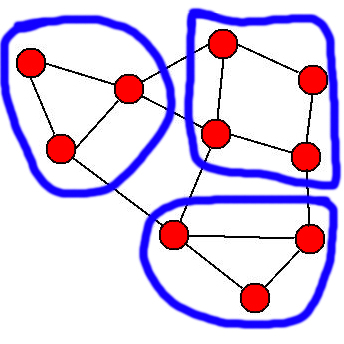
\includegraphics[width=1.0\textwidth]{aggregation.jpg} \\
				\scriptsize{clustering vertices into aggregates}
			\end{center}
		\end{column}
		\end{columns}

	\end{frame}
	
	\begin{frame}
		\frametitle{Prolongation Operator (2/2)}
		\framesubtitle{Smoothed Aggregation: Parameters}
			
			We employed a ``decoupled'' aggregation scheme:
			\vspace{0.2cm}
			\begin{itemize}
				\item aggregates of size $3^d$ in $d$ dimensions ($3 \times 3 \times 3 = 27$)
				\item each processor aggregate its portion of the grid
				\item many aggregates near inter-processor boundaries with non-optimal size
				\item number of processors determine number of aggregates: coarse problem may still be to big
				\item number of vertices is substantially reduced in every coarsening step
				%IFF: memory consumption for SA AMG prec AND linear system matrix A_0 \approx 1.5*Storage(A_0)
				\item typical operator complexity for decoupled aggregation is $1.5$
			\end{itemize}
			

	\end{frame}

	\begin{frame}
		\frametitle{Smoothing Operator and Coarse Level Solver}

		 A Chebyshev polynomial smoother is used as pre- and postsmoother:
		 \begin{itemize}
			 \item polynomial smoothers perform well for parallel solvers (R. Tuminaro and C. Tong, 2000)
			 %\item polynomial smoother do not need special matrix kernels and formats for optimal performance
			 \item profit of architecture optimized matrix vector products
			 \item polynomial smoothers are easy to parallelize
		\end{itemize}

		\pause
		\vspace{1.2cm}

		We chose to use a LU based solver as direct coarse level solver


	\end{frame}

	\begin{frame}
		\frametitle{Implementation (1/3)}

		For preconditioner setup and iterative solver we used \textsc{Trilinos}:
		\begin{itemize}
			\item \textsc{ML}: smoothed aggregation based AMG preconditioner
			\item \textsc{Epetra}: distributed matrices and vectors
			\item \textsc{Amesos}: direct coarse level solver
			\item \textsc{AztecOO}: iterative solver
		\end{itemize}

		\vspace{0.8cm}

		\opal in conjunction with Independent Parallel Particle Layer (\textsc{IPPL}) offers:
		\begin{itemize}
			\item parallel fields
			\item particle representation
			\item operators on fields
		\end{itemize}

	\end{frame}

	\begin{frame}
		\frametitle{Implementation (2/3)}
		\framesubtitle{Integration in \opal II: Solver}

		\begin{center}
		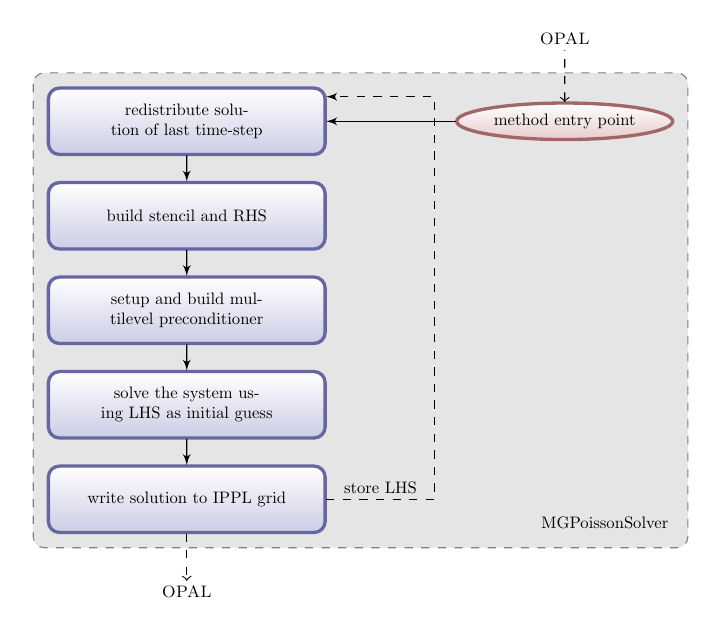
\begin{tikzpicture}[scale=0.6, transform shape, node distance = 2cm, auto]
			\tikzstyle{decision} = [diamond, draw, fill=blue!20, text width=12em, text badly centered, node distance=3cm, inner sep=0pt]
			\tikzstyle{block} = [rectangle, draw, fill=blue!20, text width=16em, text centered, rounded corners, minimum height=4em, shade,top color=white,bottom color=blue!50!black!20, draw=blue!40!black!60, very thick]
			\tikzstyle{line} = [draw, -latex'];
			\tikzstyle{cloud} = [draw, ellipse, node distance=8cm, minimum height=2em, shade, top color=white,bottom color=red!50!black!20, draw=red!40!black!60, very thick];
			
			\node [block] (redistSol) {redistribute solution of last time-step};
			\node [cloud, right of=redistSol] (entry) {method entry point};
			\node [block, below of=redistSol] (stencil) {build stencil and RHS};
			\node [block, below of=stencil] (ml) {setup and build multilevel preconditioner};
			\node [block, below of=ml] (solve) {solve the system using LHS as initial guess};
			\node [block, below of=solve] (lhs) {write solution to IPPL grid};
			%\node [decision, below of=evaluate] (decide) {is best candidate better?};
			\path [line] (redistSol) -- (stencil);
			\path [line] (stencil) -- (ml);
			\path [line] (ml) -- (solve);
			\path [line] (solve) -- (lhs);
			\path [line] (entry) -- (redistSol);
			\path [line,dashed] (lhs.east) -- node {store LHS} + (2.3,0.0) |- (redistSol.370);
			%\path [line,dashed] (lhs.east) -| node [near start] {store LHS} (redistSol.east);

			\draw [<-,dashed] (entry) -- node [above, text width=5em] {} + (0,1.5) node[above] {\opal};
			\draw [->,dashed] (lhs.270) -- node [above, text width=5em] {} + (0,-1.0) node[below] {\opal};


			\begin{pgfonlayer}{background}
        			\path (redistSol.north west)+(-0.3,0.3) node (a) {};
			        \path (lhs.south -| entry.east)+(+0.3,-0.3) node (b) {};
			        \path[fill=black!10,rounded corners, draw=black!50, dashed] (a) rectangle (b);
			        \path (lhs.east)+(5.9,-0.5) node (name) {MGPoissonSolver};
			\end{pgfonlayer}

		\end{tikzpicture}
		\end{center}

	\end{frame}

	\begin{frame}
		\frametitle{Implementation (3/3)}
		\framesubtitle{Interface between \textsc{IPPL} and \textsc{Epetra}}

		\begin{block}{\textsc{IPPL} to \textsc{Epetra} Map}
		\begin{algorithmic}[1]
			\STATE \textbf{procedure} IPPLToMap3D(localidx)

			\STATE idx $\leftarrow$ 0

			\FORALL{localidx.$x$}
				\FORALL{localidx.$y$}
					\FORALL{localidx.$z$}
						\STATE MyGlobalElements[idx] $\leftarrow$ bp$\rightarrow$getIdx($x$,$y$,$z$)
						\STATE idx $\leftarrow$ $\text{idx} + 1$
					\ENDFOR
				\ENDFOR
			\ENDFOR
			
			\RETURN \textbf{new} Epetra\_Map(-1, NumMyElements, \&MyGlobalElements[0], 0, Comm)
			\STATE \textbf{end procedure}
  		\end{algorithmic}
		\end{block}

	\end{frame}


    \section{Boundary Conditions}
	
	\begin{frame}
		\frametitle{Boundary Condition Problem}

		\begin{block}{Boundary Problem}
		Lets denote $\Omega \subset \Re^3$ the simply connected computational domain and $\Gamma= \Gamma_1 \cup \Gamma_2$, the boundary of $\Omega$ ($\Gamma_1 \cap \Gamma_2 = \emptyset$). As mentioned we solve:
		\begin{eqnarray*}
			\nabla^2 \phi = -\frac{\rho}{\epsilon_0} \text{, in } \Omega \subset \Re^3 , \nonumber \\
			\phi = 0 \text{, on }\Gamma_1   \\
			\frac{\partial \phi}{\partial \vec{n}} + \frac {1}{d} \phi = 0  \text{, on } \Gamma_2\text{,}
		\end{eqnarray*}
		with $\epsilon_0$ denotes the dielectric constant and $d$ is the distance of the bunches centroid to the  boundary.
		\end{block}
		
		\pause
		\vspace{0.3cm}
		\begin{enumerate}
			\item $\Gamma_1$ is the surface of an elliptic beam-pipe
			\item $\Gamma_1$ is the surface of an arbitrary beam-pipe element
		\end{enumerate}
	
	\end{frame}
	
	\begin{frame}
		\frametitle{Using Real Beam-Pipe Geometries}

		\begin{columns}
		\begin{column}{5cm}
			\begin{exampleblock}{Components}
			\begin{itemize}
				\item arbitrary bounded domains are specified in files
				\item \opal imports triangulated surface mesh
				\item efficient intersection of grid with surface mesh
				\item discretization approach
			\end{itemize}
			\end{exampleblock}
			\begin{block}{Motivation}
			\begin{itemize}
				\item more accurate simulation of space-charges
			\end{itemize}
			\end{block}
		\end{column}
		\begin{column}{5cm}
			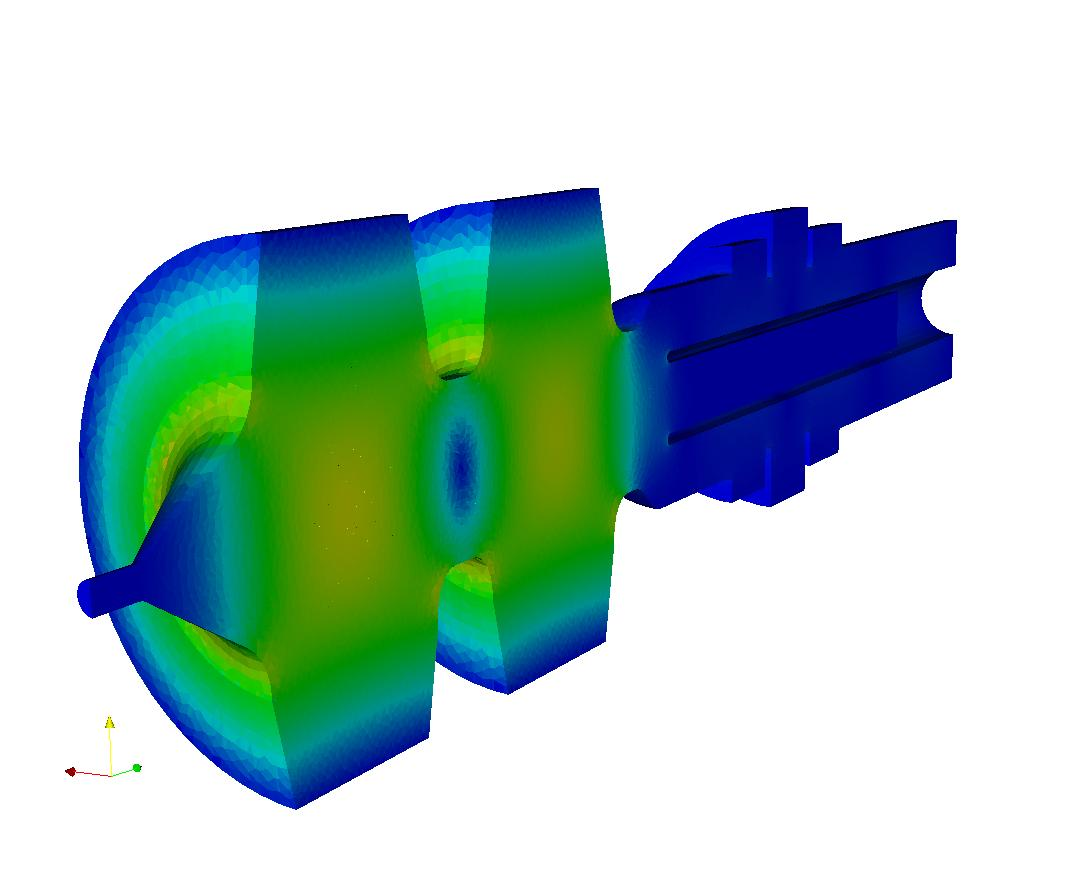
\includegraphics[width=1.0\textwidth]{electric_field_mode_4_ohne_symmetrie_v5qmm.jpg} \\
			\scriptsize{2 Frequency LEG Cavity (Based on the design of  J.-Y. Raguin (PSI))}
		\end{column}
		\end{columns}

	\end{frame}
    	
	\begin{frame}
		\frametitle{Discretization: Irregular Domains (1/2)}
		\framesubtitle{$O(h)$ Approach}

		The key idea of this approach is to only consider grid points inside the domain neglecting the distance to the domain boundary:
		\[
			(h_w^{-1}+h_s^{-1}+h_e^{-1}+h_n^{-1})u_p - h_n^{-1} u_n - h_w^{-1} u_w - h_s^{-1} u_s - h_e^{-1} \underbrace{u_e}_{=0} = f_p
		\]

		\vspace{0.5cm}
	
		\begin{alertblock}{Properties}
		\begin{itemize}
			\item the resulting discretization matrix is symmetric
			\item $O(h)$ accurate
		\end{itemize}
		\end{alertblock}

	\end{frame}
	
	\begin{frame}
		\frametitle{Discretization: Irregular Domains (2/2)}
		\framesubtitle{Shortley-Weller approximation}
	
		\begin{columns}
		\begin{column}{4cm}	
			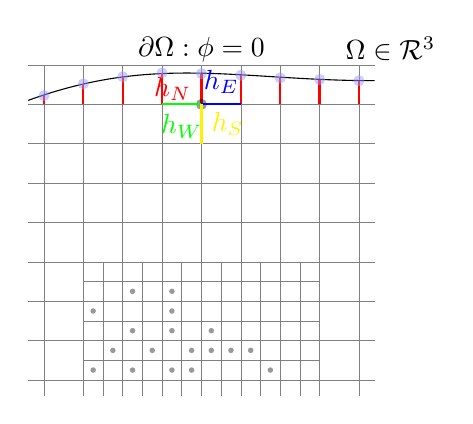
\begin{tikzpicture}[domain=-0.2:4.2,scale=1.0]
    \draw[very thin,color=gray,step=5mm] (-0.2,-0.2) grid (4.2,4);
    \draw[very thin,color=gray,step=2.5mm] (0.5,-0.2) grid (3.5,1.5);
    
    %\filldraw[fill=gray!20,fill opacity=0.8](2,2)--(2,3)--(3,3)--(3,2)--cycle;

    %curved boundart
    \draw (-0.2,3.55) to[out=20,in=180] node [sloped,below] {} (4.2,3.8);
    %\draw (-0.2,3.3) to[out=30,in=180] node [sloped,below] {$\Omega$} (4.2,3.8);
    
    %\coordinate [label=above:\C] (C) at (intersection of B and 1,0--1,1);
    %\fill[black,opacity=.5] C circle (2pt);
  
    %labels
    \node at (4.4,4.2) {$\Omega \in \mathcal{R}^3$};
    \node at (2,4.2) {$\partial \Omega: \phi = 0$};

    %interpolation lines
    \draw[thick,color=red] (0.0,3.5) to (0.0,3.61);
    \draw[thick,color=red] (0.5,3.5) to (0.5,3.76);
    \draw[thick,color=red] (1.0,3.5) to (1.0,3.85);
    \draw[thick,color=red] (1.5,3.5) to (1.5,3.90);
    \draw[thick,color=red] (2.0,3.5) to node[left] {$h_N$}(2.0,3.89);
    \draw[thick,color=red] (2.5,3.5) to (2.5,3.87);
    \draw[thick,color=red] (3.0,3.5) to (3.0,3.835);
    \draw[thick,color=red] (3.5,3.5) to (3.5,3.815);
    \draw[thick,color=red] (4.0,3.5) to (4.0,3.8);

    %on example interpol-point
    \fill[color=black,opacity=0.4] (2.0,3.5) circle (2pt);
    \draw[thick,color=green] (2.0,3.5) to node[below] {$h_W$} (1.5,3.5);
    \draw[thick,color=blue] (2.0,3.5) to node[above] {$h_E$} (2.5,3.5);
    \draw[thick,color=yellow] (2.0,3.5) to node[right] {$h_S$} (2.0,3.0);
    %\node at (2.2,3.7) {$h_{E}$};
    %\node at (1.7,3.7) {$h_{W}$};
    %\node at (2.2,3.2) {$h_{S}$};
    %\node at (2.2,3.2) {$h_{N}$};


    %short notice: dont use intersect
    \fill[blue!40,opacity=0.5] (0,3.61) circle (2pt);
    \fill[blue!40,opacity=0.5] (0.5,3.76) circle (2pt);
    \fill[blue!40,opacity=0.5] (1,3.85) circle (2pt);
    \fill[blue!40,opacity=0.5] (1.5,3.9) circle (2pt);
    \fill[blue!40,opacity=0.5] (2,3.89) circle (2pt);
    \fill[blue!40,opacity=0.5] (2.5,3.87) circle (2pt);
    \fill[blue!40,opacity=0.5] (3,3.835) circle (2pt);
    \fill[blue!40,opacity=0.5] (3.5,3.815) circle (2pt);
    \fill[blue!40,opacity=0.5] (4,3.8) circle (2pt);

    %particles
    \fill[black!40] (0.625,0.125) circle (1pt);
    \fill[black!40] (0.625,0.875) circle (1pt);
    
    \fill[black!40] (0.875,0.375) circle (1pt);

    \fill[black!40] (1.625,1.125) circle (1pt);
    
    \fill[black!40] (1.375,0.375) circle (1pt);

    \fill[black!40] (1.125,1.125) circle (1pt);
    \fill[black!40] (1.125,0.625) circle (1pt);
    \fill[black!40] (1.125,0.125) circle (1pt);
    
    \fill[black!40] (1.625,0.875) circle (1pt);
    \fill[black!40] (1.625,0.125) circle (1pt);
    \fill[black!40] (1.625,0.625) circle (1pt);

    \fill[black!40] (1.875,0.375) circle (1pt);
    \fill[black!40] (1.875,0.125) circle (1pt);
    
    \fill[black!40] (2.125,0.375) circle (1pt);
    \fill[black!40] (2.125,0.625) circle (1pt);

    \fill[black!40] (2.375,0.375) circle (1pt);

    \fill[black!40] (2.625,0.375) circle (1pt);
    
    \fill[black!40] (2.875,0.125) circle (1pt);

\end{tikzpicture}

		\end{column}
		\begin{column}{6.5cm}	
		\small{	
			\[
				2 \begin{bmatrix}
				& \frac{b}{h_N (h_N + h_S)} & \\
				\frac{a}{h_W (h_W + h_E)} & -\frac{a}{h_w h_E} -\frac{b}{h_S h_N} & \frac{a}{h_E (h_W + h_E)} \\
				& \frac{b}{h_S (h_N + h_S)} & \\
				\end{bmatrix}_h
			\] 
		}
		\end{column}
		\end{columns}
		
		\begin{alertblock}{Properties}
		\begin{itemize}
			\item the resulting discretization matrix is non-symmetric for boundary points
			\item $O(h^2)$ accurate
		\end{itemize}
		\end{alertblock}

	\end{frame}

	\begin{frame}
		\frametitle{Implementation (1/2)}
		\framesubtitle{Importing geometries in \opal}

		\begin{center}
			\tikzstyle{format} = [draw, thin, fill=blue!20]
\tikzstyle{pblock} = [rectangle, draw, fill=blue!20, text width=6em, text centered, rounded corners, minimum height=0.4em]
\tikzstyle{mblock} = [rectangle, draw, fill=green!20, text width=6em, text centered, rounded corners, minimum height=0.4em]
\tikzstyle{bblock} = [rectangle, draw, fill=gray!20, text width=6em, text centered, rounded corners, minimum height=0.4em]
\tikzstyle{prblock} = [rectangle, draw, fill=red!20, text width=6em, text centered, rounded corners, minimum height=0.4em]
\tikzstyle{rblock} = [rectangle, draw, fill=olive!20, text width=6em, text centered, rounded corners, minimum height=0.4em]
%\tikzstyle{block} = [rectangle, draw, fill=blue!20, text centered, rounded corners]
\tikzstyle{decision} = [diamond, draw, fill=blue!20, text width=4.5em, text badly centered, node distance=3cm, inner sep=0pt]
\tikzstyle{medium} = [ellipse, draw, thin, fill=green!20, minimum height=2.5em]
\tikzstyle{cloud} = [draw, ellipse,fill=red!20, node distance=3cm, minimum height=2em]
\tikzstyle{line} = [draw, -latex']
\tikzstyle{emptyblock} = [rectangle]


\begin{tikzpicture}[scale=0.8,transform shape,node distance=3cm]%[node distance = 3cm, scale=0.5]
    % Place nodes
    \node [pblock] (STEP) {
		     STEP file};
    \node [bblock, right of=STEP] (BOGUI) {
		     heronion};
    \node [mblock, right of=BOGUI] (surfmesh) {
		     surface mesh};
    \node [mblock, below of=surfmesh] (add) {
		     mesh, ...};
    \node [pblock, right of=surfmesh] (H5FED) {
		     H5FED};
    \node [pblock, above of=H5FED] (H5Part) {
		     H5Part};

    \node [pblock, below of=H5FED] (VTK) {
    		     VTK};
    \node [bblock, right of=H5FED] (OPAL) {
    		     OPAL};
		  
    % Draw edges
    \path [line] (STEP) -> (BOGUI);
    \path [line] (BOGUI) -> (surfmesh);
    \path [line,style=dashed, ->] (BOGUI) edge [out=-90, in=90] (add);
    \path [line] (surfmesh) -> (H5FED);
    \path [line,style=dashed, ->] (surfmesh) edge [out=-90, in=90] (VTK);
    %\path [->] (fifth) edge [out=-90, in=90] (distmesh);
    \path [->] (H5FED) edge (OPAL);
    \path [line,style=dashed, ->] (H5FED) edge [out=90, in=180] node[right] {part of} (H5Part);
    \path [<->] (H5Part) edge [out=0, in=90] (OPAL);
    

\end{tikzpicture}

%\begin{tikzpicture}[overlay]
%	\path[->]<1-> (third) (fifth);
%	\path[->,red!40,thick]<2-> (second) edge [bend right] (fifth);
%\end{tikzpicture}

		\end{center}

		\small{in collaboration with B. Oswald and A. Gsell (AIT)}

	\end{frame}
	
	\begin{frame}
		\frametitle{Implementation (2/2)}
		\framesubtitle{Setup Phase}

		\begin{columns}
		\begin{column}{6.6cm}
		\begin{itemize}
			\item extended \textsc{Heronion} to dump H5Fed surface mesh
			\item \opal imports H5Fed files (serial): $m$ triangles and $v$ vertices
			\item efficient intersection of grid-lines with triangular surface mesh (T. Moeller and B. Trumbore (1997)): 
				\begin{itemize}
					\item arbitrary domain: $O(m(n_x+n_y+local_z))$ 
					\item elliptic domain: $O(n_x + n_y)$
				\end{itemize}
			\item building index table
				\begin{itemize}
					\item arbitrary domain: $O(n_x n_y local_z)$
					\item elliptic domain: $O(n_x n_y)$
				\end{itemize}
		\end{itemize}
		\end{column}
		\begin{column}{4cm}	
			\begin{center}
			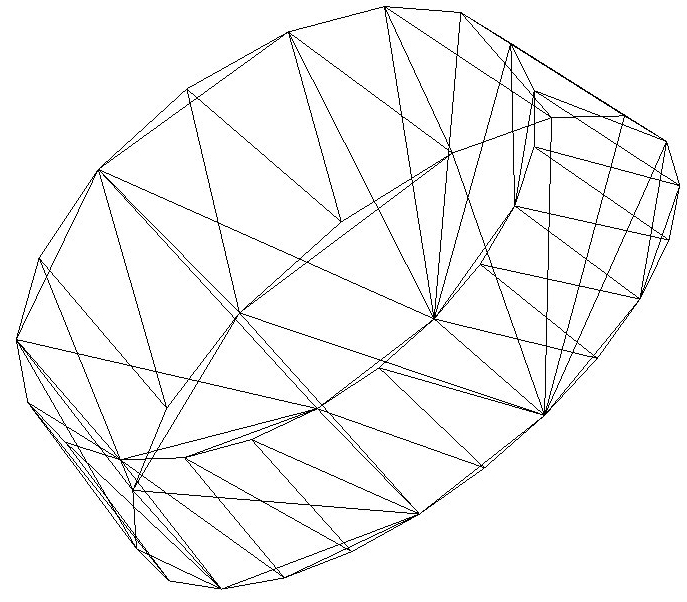
\includegraphics[width=1.0\textwidth]{cylinder.jpg}
			\end{center}
		\end{column}
		\end{columns}

	\end{frame}

     \section{Results}

     	\begin{frame}
		\frametitle{Environment}

		\begin{exampleblock}{Buin: Cray XT4 cluster at the CSCS in Manno}
		\begin{itemize}
			\item 468 AMD dual core Opteron at 2.6 GHz
			\item 936 GB DDR RAM
			\item 30 TB Disk
			\item 7.6 GB/s interconnect bandwith
		\end{itemize}
		\end{exampleblock}
		\pause

		\begin{center}
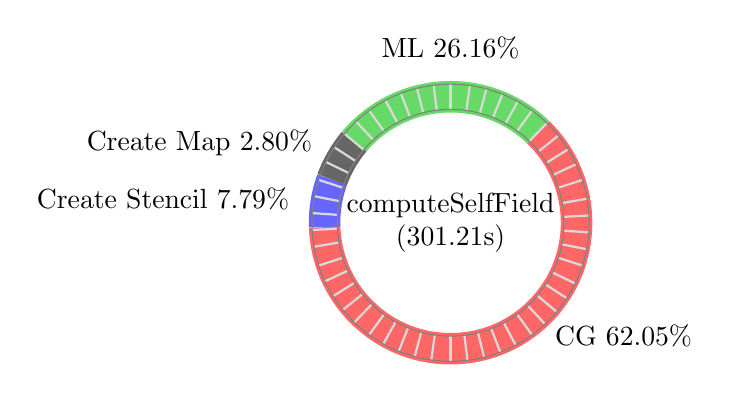
\begin{tikzpicture}[scale=0.8]
  \colorlet{CRSTENCIL}{blue!60!white}
  \colorlet{ML}{green!75!black!60!white}
  \colorlet{CG}{red!60!white}
  \colorlet{RECALCMAP}{black!60}

  \node[text centered,text width=3cm]{computeSelfField (301.21s)};

  \begin{scope}[line width=4mm,rotate=270]
    \draw[CRSTENCIL]	(-110:2cm) arc (-110:-88:2cm);
    \draw[CG]	        (-88:2cm) arc (-88:136:2cm);
    \draw[ML]           (136:2cm)  arc (136:230:2cm);
    \draw[RECALCMAP]	(230:2cm) arc (230:250:2cm);

    \newcount\mycount
    \foreach \angle in {0,72,...,3599}
    {
      \mycount=\angle\relax
      \divide\mycount by 10\relax
      \draw[black!15,thick] (\the\mycount:18mm) -- (\the\mycount:22mm);
    }
    
    \draw (180:2.2cm) node[above] {ML 26.16\%};
    \draw (-100:2.2cm) node[left] {Create Stencil 7.79\%};
    \draw (-125:2.2cm) node[left] {Create Map 2.80\%};
    \draw (35:2.2cm) node[right] {CG 62.05\%};
  \end{scope}  
  \draw[gray] (0,0) circle (2.2cm) circle (1.8cm);
\end{tikzpicture}
		\end{center}

	\end{frame}

     	\begin{frame}
		\frametitle{Validation}

		For validation purposes we defined a to the $z$ axis, rotation symmetric potential function and calculated the analytical solution.

		\vspace{0.5cm}

		Arbitrary domains: tested with a triangulated surface mesh of a cylinder with the same potential function.

		\vspace{0.7cm}
		\pause

		\textbf{Results}: $L_2$ norms of the error:
		\begin{center}
			\rowcolors{1}{blue!20}{blue!5}
			\begin{tabular}{|c|c|c|}
			\hline
			grid size & elliptic & arbitrary \\
			\hline
			$20 \times 20 \times 20$ & $0.1158$ & $0.1145$ \\
			$40 \times 40 \times 40$ & $0.0846$ & $0.0838$ \\
			$80 \times 80 \times 80$ & $0.0765$ & $0.0755$ \\
			%domain & discretization & $L_2$ norm of error \\
			%\hline
			%elliptic & OH & 0.0617 \\
			%elliptic & SW & 0.0571 \\
			%arbitrary & SW & 0.0572 \\
			\hline
        		\end{tabular}
		\end{center}

	\end{frame}

	%\begin{frame}
	%	\frametitle{Convergence (1/2)}
	%	\framesubtitle{$O(h)$}

	%	On a $256 \times 256 \times 2048$ grid:
	%	\begin{center}
	%	\rowcolors{1}{blue!20}{blue!5}
	%	\begin{tabular}{|l|l|l|}
	%	\hline
	%		domain & number of nodes & iterations \\
	%		\hline
	%		elliptic & $128$ & $12$  \\
	%		elliptic & $256$ & $12$  \\
	%		elliptic & $512$ & $11$  \\
	%		\hline
	%		arbitrary & $128$ & ? \\
	%		arbitrary & $256$ & ? \\
	%		arbitrary & $512$ & ? \\
	%		\hline
	%	\end{tabular}
	%	\end{center}


	%\end{frame}
	
	\begin{frame}
		\frametitle{Convergence}

		On a $256 \times 256 \times 2048$ grid:
		\begin{center}
		\rowcolors{1}{blue!20}{blue!5}
		\begin{tabular}{|l|l|l|l|}
			\hline
			discretization & number of nodes & iter. for CG & iter. for BiCGStab\\
			\hline
			$O(h)$ & $128$ & $12$ & - \\
			$O(h)$ & $256$ & $12$ & - \\
			$O(h)$ & $512$ & $11$ & - \\
			\hline
			SW & $128$ & $17$ & $10$ \\
			SW & $256$ & $17$ & $10$ \\
			SW & $512$ & $18$ & $11$ \\
			%\hline
			%arbitrary & $128$ & ? & ? \\
			%arbitrary & $256$ & ? & ? \\
			%arbitrary & $512$ & ? & ? \\
			\hline
		\end{tabular}
		\end{center}

	\end{frame}
	
	\begin{frame}
		\frametitle{Parallel Efficiency (1/2)}
		\framesubtitle{Timings}

		\begin{center}
		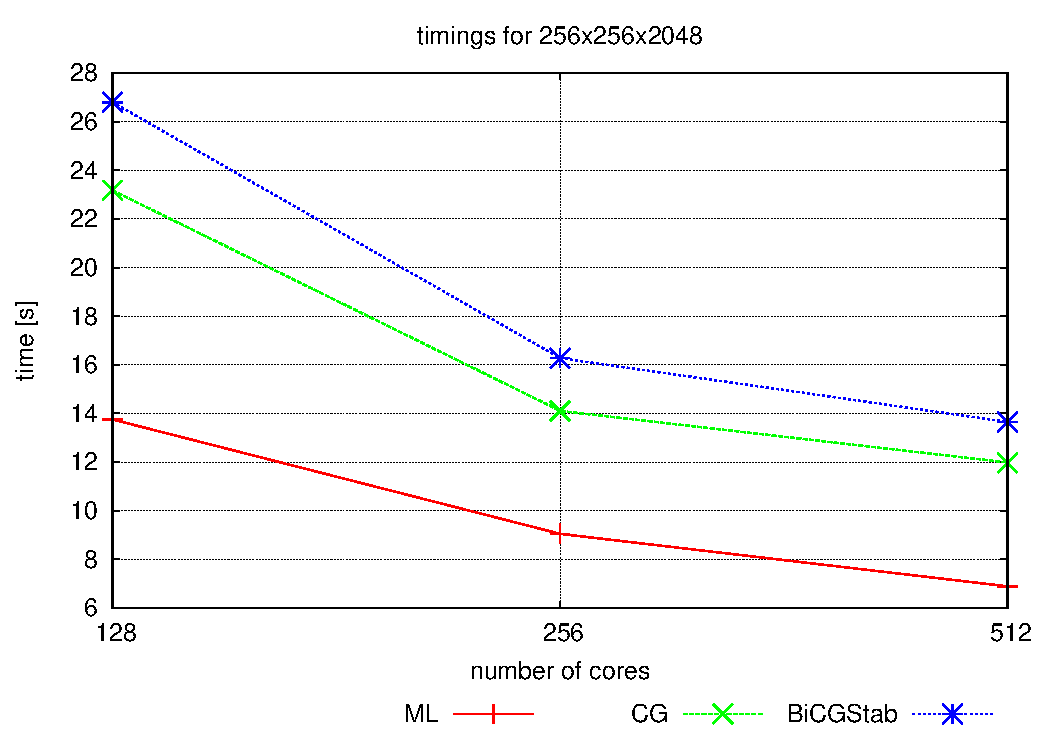
\includegraphics[width=0.9\textwidth]{plots/timings_SW.pdf}
		\end{center}

	\end{frame}
	
	\begin{frame}
		\frametitle{Parallel Efficiency (2/2)}
		\framesubtitle{Speedup}
		
		\begin{center}
		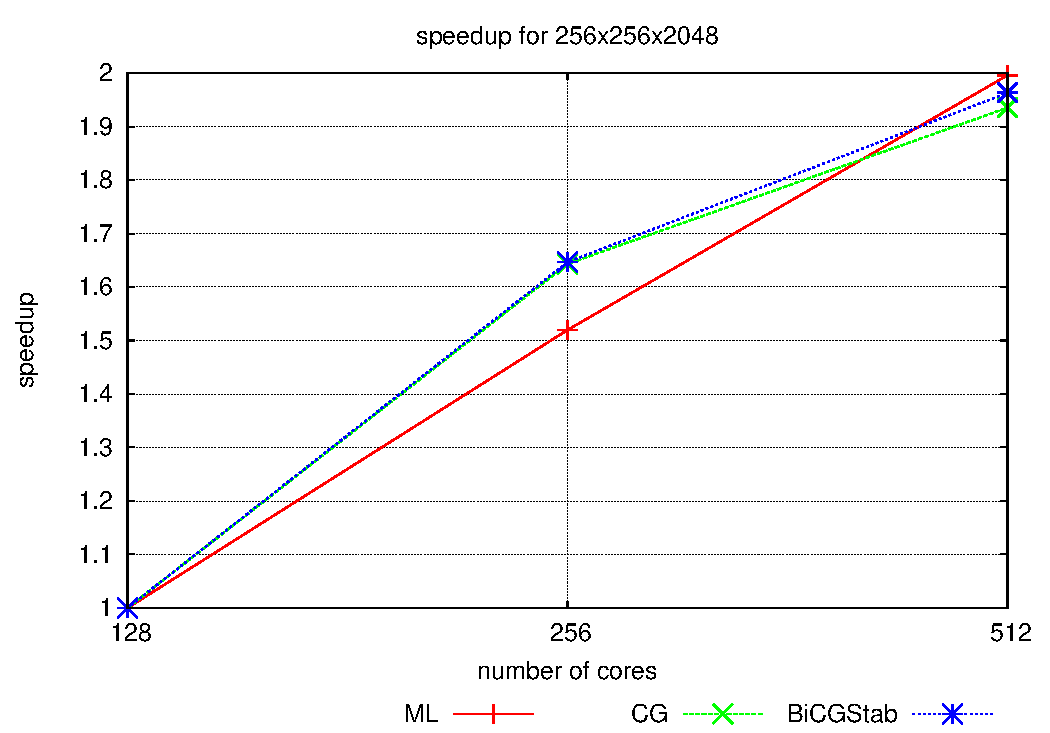
\includegraphics[width=0.9\textwidth]{plots/speedup_SW.pdf}
		\end{center}

	\end{frame}


     \section{Summary}

     	\begin{frame}
		\frametitle{Summary}

		\textbf{Improved Space-Charge Solver:} \\

		\begin{itemize}
			\item is discretized with finite differences
			\item smoothed aggregation based algebraic Multigrid preconditioner
			\item fully integrated into \opal 
			\item reuse solutions of previous time-steps
		\end{itemize}
		\pause

		\vspace{0.4cm}

		\textbf{Improved Boundary Conditions:} \\

		\begin{itemize}
			\item Shortley-Weller approximation
			\item elliptic beam-pipe domain
			\item arbitrary domains based on real geometries of beam-pipe elements
			\item beam-pipe geometries can be processed and imported
		\end{itemize}

	\end{frame}

	\begin{frame}
		\frametitle{Problems and Further Work}

		\begin{alertblock}{Problems}
		\begin{itemize}
			\item \opal on Buin cluster in Manno: stand-alone solver
			\item ACML
		\end{itemize}
		\end{alertblock}
		\pause

		\vspace{0.8cm}

		\begin{block}{Further Work}
		\begin{itemize}
			\item parallelize in $x$ and $y$ direction
			\item validation of arbitrary domains against complex geometries
			\item investigate in non-symmetry solver
			\item improve aggregation process
			\item adaptive mesh refinement (AMR)
		\end{itemize}
		\end{block}

	\end{frame}
 
	\begin{frame}
	  	\frametitle{Backup}
		\begin{center}
			\color{blue}{\LARGE{Backup}}
		\end{center}
	\end{frame}

	\begin{frame}
		\frametitle{Implementation (2/4)}
		\framesubtitle{Integration in \opal I: Class Hierarchy}

		\begin{center}
		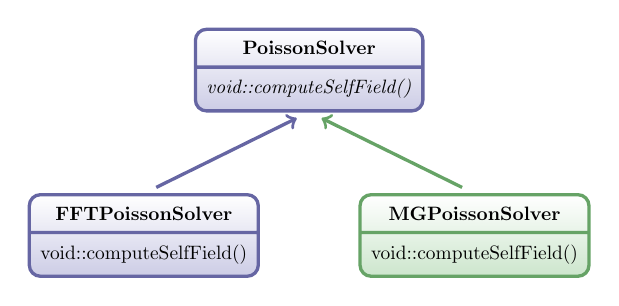
\begin{tikzpicture}[scale=0.7, transform shape, grow=down, level 1/.style={sibling distance=6cm,level distance=3cm},edge from parent/.style={very thick,draw=blue!40!black!60,shorten >=5pt, shorten <=5pt},edge from parent path={(\tikzparentnode.south) -- (\tikzchildnode.north)},every node/.style={text ragged, inner sep=2mm}]

			\tikzstyle{class} = [rectangle, rounded corners, shade, top color=white,bottom color=blue!50!black!20, draw=blue!40!black!60, very thick];
			\tikzstyle{newclass} = [rectangle, rounded corners, shade, top color=white,bottom color=green!50!black!20, draw=green!40!black!60, very thick];

			\node[class] [rectangle split, rectangle split, rectangle split parts=2, text ragged] {
			    \textbf{PoissonSolver}
			    \nodepart{second} 
			    	\textit{void::computeSelfField()}
			}
			    child {
			        node[class] [rectangle split, rectangle split parts=2, text ragged] {
			            \textbf{FFTPoissonSolver}
			            \nodepart{second} 
				      void::computeSelfField() 
			        }
		        edge from parent [<-]
		    }
			    child {
			    	node[newclass] [rectangle split, rectangle split parts=2, text ragged] {
				    \textbf{MGPoissonSolver}
				    \nodepart{second} 
				      void::computeSelfField() 
				}
		        edge from parent [<-, draw=green!40!black!60]
		   };
		\end{tikzpicture}
		\end{center}

	\end{frame}

	\begin{frame}
		\frametitle{Implementation (1/3)}
		\framesubtitle{Class Diagram}

		\begin{center}
		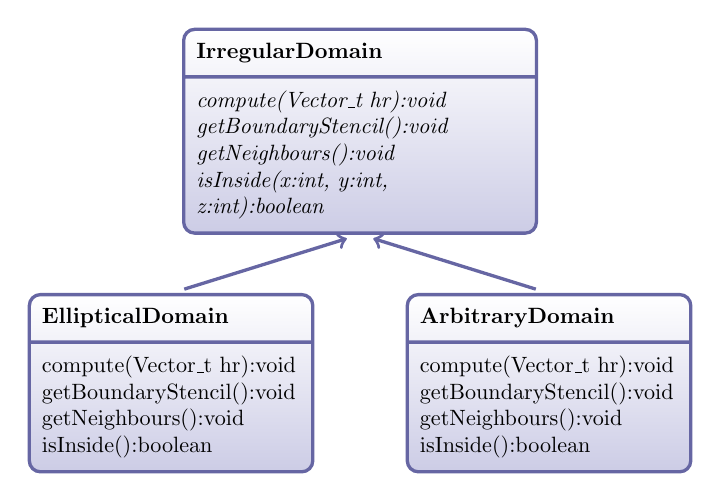
\begin{tikzpicture}[scale=0.8, transform shape, grow=down, level 1/.style={sibling distance=6cm,level distance=4cm},edge from parent/.style={very thick,draw=blue!40!black!60,shorten >=5pt, shorten <=5pt},edge from parent path={(\tikzparentnode.south) -- (\tikzchildnode.north)},every node/.style={text ragged, inner sep=2mm}]

\tikzstyle{class} = [rectangle, rounded corners, shade, top color=white,bottom color=blue!50!black!20, draw=blue!40!black!60, very thick];

\node[class] [rectangle split, rectangle split parts=2, text width=5.2cm] {
    \textbf{IrregularDomain}
    \nodepart{second} 
    	\textit{compute(Vector\_t hr):void} \\
	\textit{getBoundaryStencil():void} \\
	\textit{getNeighbours():void} \\
	\textit{isInside(x:int, y:int, z:int):boolean}
    }
    child {
        node[class] [rectangle split, rectangle split parts=2, text width=4.1cm] {
            \textbf{EllipticalDomain}
            \nodepart{second} 
	      compute(Vector\_t hr):void \\
	      getBoundaryStencil():void \\
	      getNeighbours():void \\
	      isInside():boolean
        }
        edge from parent [<-]
    }
    child {
    	node[class] [rectangle split, rectangle split parts=2, text width=4.1cm] {
	    \textbf{ArbitraryDomain}
	    \nodepart{second} 
	      compute(Vector\_t hr):void \\
	      getBoundaryStencil():void \\
	      getNeighbours():void \\
	      isInside():boolean
	}
        edge from parent [<-]
   };
\end{tikzpicture}
\end{center}


	\end{frame}


	\begin{frame}
		\frametitle{SW: non-symmetries}

		\begin{center}
		    \begin{tikzpicture}[domain=-0.2:4.2,scale=1.4]
    \draw[very thin,color=gray,step=10mm] (-0.2,-0.2) grid (4.2,4.2);
    
    %curved boundart
    \draw (0,0) to[out=90,in=180] node [sloped,below] {} (2,4);
  
    \node at (4.6,4.2) {$\Omega \subset \Re^3$};
    \node at (-0.8,2.5) {$\partial \Omega: \phi = 0$};

    \draw[thick,color=red] (0.18,2) to node[above] {$G_w$}(1,2);
    \draw[thick,color=red] (0.48,3) to node[below] {$H_w$}(1,3);

    \fill[blue!60,opacity=0.5] (1,2) node[right] {$G$} circle (2pt);
    \fill[blue!60,opacity=0.5] (1,3) node[right] {$H$} circle (2pt);

\end{tikzpicture}

		\end{center}

	\end{frame}
	
	\begin{frame}
		\frametitle{Grid Operators}
		\framesubtitle{AMG: smoothed aggregation}

		%TODO: finish

		Operate on directly on (linear sparse) algebraic equations:

		\[
			\sum_j a_{ij}^h x_j^h = b_i^h
		\]

		\begin{itemize}
			\item replace "grid" with "variables"
			%\item AMG fixes smoother and adjusts coarsening (GMG inverse)
			\item coarse level equations are generated without the use of any geometry
			\item no coarse level grids have to be generated or stored
			\item good preconditioner: works on all error components (in contrast to level-one preconditioner)
		\end{itemize}

		\vspace{0.2cm}
		SA restrict operator:

		\[
			I_H^h = (I_h - \omega D_h^{-1} A_h^f) \hat{I}_H^h
		\]

		%generate operator dependet interpolation and Galerkin operator can be derived directly from the underlying matrices, without any reference to the actual grids.
	
  	\end{frame}

    	\begin{frame}
		\frametitle{Multigrid Theory (1/2)}
		\framesubtitle{Motivation}

		\begin{block}{Important Observations}
			\begin{itemize}
				\item Some classical iterative methods (i.e. Gauss Seidel) have a smoothing effect on the error of any approximation for discrete elliptic problems.
				\vspace{0.2cm}
				\item A smooth error can be well approximated on a coarse grid. This coarse grid has considerably fewer grid points and is therefore cheaper to solve.
			\end{itemize}
		\end{block}

		\vspace{0.4cm}

		From this two observations a Two-Grid can be deduced:

		\begin{enumerate}
			\item apply smoother
			\item restrict to a grid with considerably fewer grid points (coarse)
			\item solve
			\item interpolate back to the fine grid
			\item compute a new approximation
		\end{enumerate}

	\end{frame}
    	
	\begin{frame}
		\frametitle{Multigrid Theory (2/2)}
		\framesubtitle{The Two-Grid: Smoothed Coarse Grid Correction}

		The discretized system is solved by a Two-Grid:

		\[
			A\mathbf{x} = \mathbf{b}
		\]
		\[
			e_h^m = x_h - x_h^m\text{, } r_h^m = b_h - A_hx_h^m
		\]
		\[
			r_h^m = A_h e_h^m
		\]

		\vspace{0.1cm}

		\begin{center}
		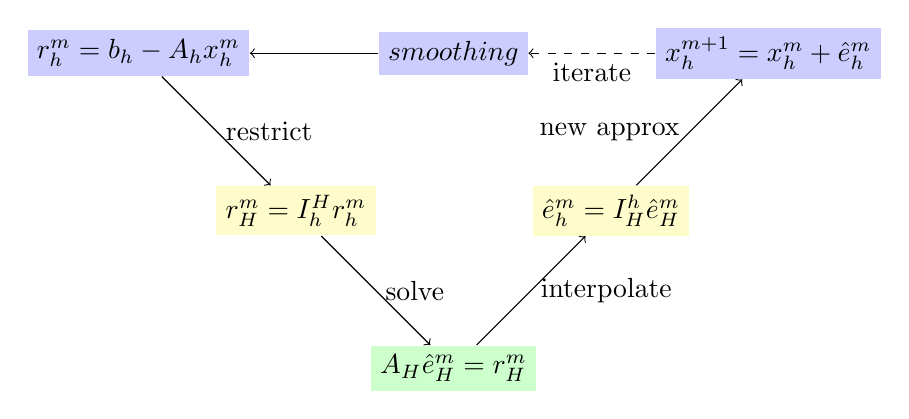
\begin{tikzpicture}[scale=1,transform shape,node distance=2cm]	
            		\node[fill=blue!20] (res)
            		{$ r_h^m = b_h - A_h x_h^m $};
			\node[right of=res] (dummy6) {};
            		\node[fill=blue!20, right of=dummy6] (smooth)
            		{$ smoothing $};
			\node[below of=res] (dummy1) {};
            		\node[fill=yellow!20, right of=dummy1] (restrict)
            		{$ r_H^m = I_h^H r_h^m$};
			\node[below of=restrict] (dummy2) {};
            		\node[fill=green!20, right of=dummy2] (solve)
            		{$ A_H \hat{e}_H^m = r_H^m $};
			\node[right of=solve] (dummy3) {};
            		\node[fill=yellow!20, above of=dummy3] (interpolate)
            		{$ \hat{e}_h^m = I_H^h \hat{e}_H^m $};
			\node[right of=interpolate] (dummy4) {};
            		\node[fill=blue!20, above of=dummy4] (newapprox)
			{$ x_h^{m+1} = x_h^m + \hat{e}_h^m $};

        		\path[->] (res) edge node[right] {restrict} (restrict);
        		\path[->] (restrict) edge node[right] {solve} (solve);
        		\path[->] (solve) edge node[right] {interpolate} (interpolate);
        		\path[->] (interpolate) edge node[left] {new approx} (newapprox);
        		\path[->] (smooth) edge (res);
        		\path[->,dashed] (newapprox) edge node[below] {iterate} (smooth);
		\end{tikzpicture}
		\end{center}

	\end{frame}

	\begin{frame}
		\frametitle{Grid Operators}
		\framesubtitle{Geometric Multigrid}

		\begin{columns}
		\begin{column}{4.5cm}
		\textbf{restriction} \\
		\vspace{0.4cm}
		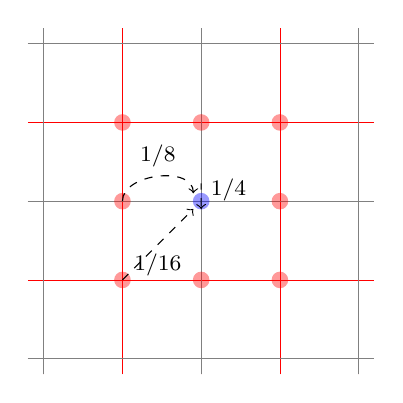
\begin{tikzpicture}[scale=1.0,transform shape,node distance=1cm]	
			\draw[very thin,color=red,step=1cm] (-0.2,-0.2) grid (4.2,4.2);
			\draw[very thin,color=gray,step=2cm] (-0.2,-0.2) grid (4.2,4.2);
			
			%\draw[very thin,color=gray,step=2cm] (5,-0.2) grid (9.2,4.2);
    
			\fill[color=blue,opacity=0.4] (2.0,2.0) circle (3pt);
			\fill[color=red,opacity=0.4] (1.0,2.0) circle (3pt);
			\fill[color=red,opacity=0.4] (1.0,1.0) circle (3pt);
			\fill[color=red,opacity=0.4] (2.0,1.0) circle (3pt);
			\fill[color=red,opacity=0.4] (3.0,2.0) circle (3pt);
			\fill[color=red,opacity=0.4] (2.0,3.0) circle (3pt);
			\fill[color=red,opacity=0.4] (3.0,3.0) circle (3pt);
			\fill[color=red,opacity=0.4] (1.0,3.0) circle (3pt);
			\fill[color=red,opacity=0.4] (3.0,1.0) circle (3pt);
			
    			\path[style=dashed, ->] (1.0,2.0) edge [out=90, in=90] node[above] {\footnotesize{$1/8$}} (1.9,2.1);
    			\path[style=dashed, ->] (1.0,1.0) edge node[below] {\footnotesize{$1/16$}} (1.9,1.9);
    			\path[style=dashed, ->] (2.0,2.2) edge [out=90, in=91] node[right] {\footnotesize{$1/4$}} (2.0,1.9);

		\end{tikzpicture}
		\end{column}

		\begin{column}{4.5cm}
		\textbf{bilinear interpolation} \\
		\vspace{0.4cm}
		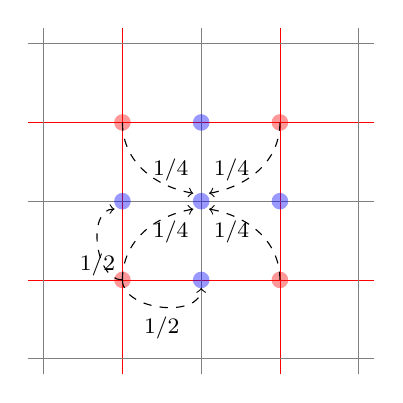
\begin{tikzpicture}[scale=1.0 ,transform shape,node distance=1cm]	
			\draw[very thin,color=red,step=1cm] (-0.2,-0.2) grid (4.2,4.2);
			\draw[very thin,color=gray,step=2cm] (-0.2,-0.2) grid (4.2,4.2);
			
			%\draw[very thin,color=gray,step=2cm] (5,-0.2) grid (9.2,4.2);
    
			\fill[color=blue,opacity=0.4] (2.0,2.0) circle (3pt);
			\fill[color=blue,opacity=0.4] (1.0,2.0) circle (3pt);
			\fill[color=red,opacity=0.4] (1.0,1.0) circle (3pt);
			\fill[color=blue,opacity=0.4] (2.0,1.0) circle (3pt);
			\fill[color=blue,opacity=0.4] (3.0,2.0) circle (3pt);
			\fill[color=blue,opacity=0.4] (2.0,3.0) circle (3pt);
			\fill[color=red,opacity=0.4] (3.0,3.0) circle (3pt);
			\fill[color=red,opacity=0.4] (1.0,3.0) circle (3pt);
			\fill[color=red,opacity=0.4] (3.0,1.0) circle (3pt);
			
    			
			\path[style=dashed, ->] (3.0,3.0) edge [out=-90, in=10] node[left] {\footnotesize{$1/4$}} (2.1,2.1);
    			\path[style=dashed, ->] (1.0,3.0) edge [out=-90, in=170] node[right] {\footnotesize{$1/4$}} (1.9,2.1);
    			\path[style=dashed, ->] (3.0,1.0) edge [out=90, in=-10] node[left] {\footnotesize{$1/4$}} (2.1,1.9);
    			\path[style=dashed, ->] (1.0,1.0) edge [out=90, in=-170] node[right] {\footnotesize{$1/4$}} (1.9,1.9);

    			\path[style=dashed, ->] (1.0,1.0) edge [out=-90, in=-90] node[below] {\footnotesize{$1/2$}} (2.0,0.9);
    			\path[style=dashed, ->] (1.0,1.0) edge [out=180, in=180] node[below] {\footnotesize{$1/2$}} (0.9,1.9);
		\end{tikzpicture}
		\end{column}
		\end{columns}

	\end{frame}
	

	\begin{frame}
		\frametitle{Multigrid}
		\framesubtitle{from Two-Grid to Multigrid}

		%v -> V / W (etc)
		\begin{center}
		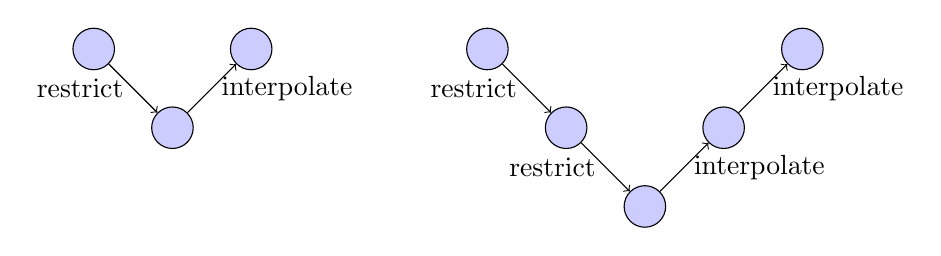
\begin{tikzpicture}[scale=1,transform shape,node distance=1cm]	
			\tikzstyle{circ} = [circle, draw, thin, fill=blue!20, minimum height=1.5em]

			%v
			\node[circ] (v1) {};
			\node[right of=v1] (dummy1) {};
			\node[circ,below of=dummy1] (v2) {};
			\node[circ,right of=dummy1] (v3) {};
        		\path[->] (v1) edge node[left] {restrict} (v2);
        		\path[->] (v2) edge node[right] {interpolate} (v3);
			
			%V
			\node[right of=v3] (DD) {};
			\node[right of=DD] (D) {};
			\node[circ,right of=D] (V1) {};
			\node[right of=V1] (Dummy1) {};
			\node[circ,below of=Dummy1] (V2) {};
			\node[right of=V2] (Dummy2) {};
			\node[circ,below of=Dummy2] (V3) {};
			\node[circ,right of=Dummy2] (V4) {};
			\node[above of=V4] (Dummy3) {};
			\node[circ,right of=Dummy3] (V5) {};
			
        		\path[->] (V1) edge node[left] {restrict} (V2);
        		\path[->] (V2) edge node[left] {restrict} (V3);
        		\path[->] (V3) edge node[right] {interpolate} (V4);
        		\path[->] (V4) edge node[right] {interpolate} (V5);
        		
		\end{tikzpicture}
		\end{center}

		\vspace{0.3cm}

		Depending on how the recursion is coded, some variants of the V-cycle can be produced.

		\begin{itemize}
			\item grid-independence convergence 
			\item iterative solver: reuse information
			\item $\mathcal{O}(n)$ algorithm
		\end{itemize}
			
		\textbf{Anisotropy} is handled in the discretized problem

	\end{frame}

%	\appendix
%	\begin{frame}
%	  \frametitle<presentation>{References}
%	  \begin{thebibliography}{10}
%	  \beamertemplatearticlebibitems
%	
%	  \bibitem{BAISU2005}
%	    Z.\ Bai. \scriptsize{AND} \normalsize{Y.\ Su.}
%	    \newblock {\em SOAR: A Second-Order Arnoldi Method for the Solution of the Quadratic Eigenvalue Problem}.
%	    \newblock SIAM J. Matrix Anal. Appl., 2005.
%
%	  \bibitem{PRESVAR}
%	    \textbf{L.\ Lee.}, L.\ Ge., Z.\ Li., C.\ Ng., K.\ Ko., B.\ Liao., Z.\ Bai., D.\ Gao., W.\ Gao., C.\ Yang., P.\ Husbands., E.G.\ Ng.
%	    \newblock{\em Solving Nonlinear Eigenproblems in Acclerator Cavity Design}.
%	    \newblock SIAM Annual Meeting, MS 44 and MS 56: Nonlinear Eigenvalue Problems, 2005
%	    
%	  \end{thebibliography}
%	\end{frame}

\end{document}
